To address the problem of engaging students in STEM education, we propose an interactive and demonstrative system that showcases practical applications of technology in an educational setting. The system will be designed to be both engaging and educational, demonstrating fundamental principles of electronics, optics, and computing in a tangible and enjoyable manner.

At a high level, the system consists of several major components that work together seamlessly to create an interactive experience. The core components include a set of lasers, phototransistors, a signal processing unit (Raspberry Pi), and an audio output system.

Major System Components:

Lasers:
These will be positioned at the bottom of the system setup. Each laser corresponds to a different 'string' in our system, akin to a musical instrument. The lasers emit continuous beams of light upwards towards corresponding phototransistors.

Phototransistors:
Placed at the top of the setup, these sensors are aligned with the lasers. Each phototransistor detects the presence of a laser beam. When a laser beam is interrupted (e.g., by a user blocking it or 'plucking' it), the corresponding phototransistor will no longer detect the light.

Signal Processing Unit (Raspberry Pi):
The Raspberry Pi acts as the brain of the system. It is responsible for receiving signals from the phototransistors, processing these signals to determine which laser beam has been interrupted, and subsequently triggering the appropriate response. The Raspberry Pi is programmed to recognize which phototransistor has detected a change and maps this change to a specific audio output.

Audio Output System:
Connected to the Raspberry Pi, this system plays a pre-recorded sound corresponding to the interrupted laser. Each laser and phototransistor pair is associated with a unique sound, which is played to provide immediate auditory feedback to the user, making the interaction engaging and informative.

User Interaction:

Users interact with the system by interrupting the laser beams. For example, a user might wave their hand through a beam or use an object to block the light. When the laser beam is interrupted, the corresponding phototransistor sends a signal to the Raspberry Pi, which processes this input and plays the associated sound. This immediate feedback loop helps users understand the cause-and-effect relationship between their actions and the system's response, reinforcing learning through interaction.

High-Level Diagram:
\begin{figure}[h!]
	\centering
   	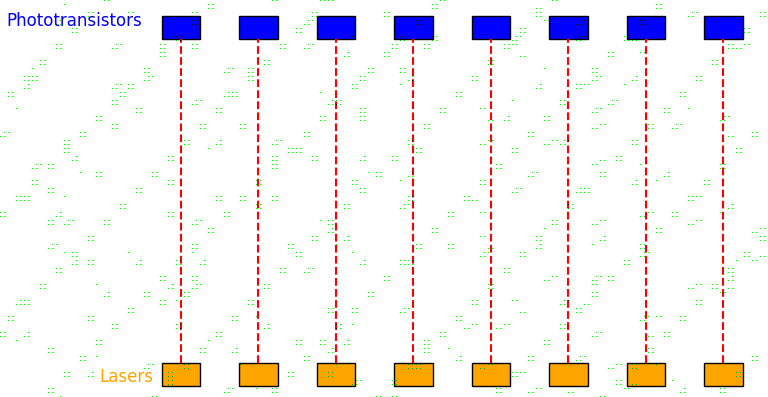
\includegraphics[width=0.60\textwidth]{images/Design.png}
\end{figure}

Each laser is aligned with a phototransistor, creating a vertical beam of light. The phototransistors detect the presence of the laser beams and send signals to the Raspberry Pi when a beam is interrupted. The Raspberry Pi then processes these signals and triggers the corresponding sound through the audio output system.

This high-level overview demonstrates how the system components interact to create an engaging and educational experience for users. By incorporating elements of electronics, optics, and computing, the project not only provides a fun and interactive way for students to engage with STEM concepts but also serves as a practical demonstration of these principles in action.
